\documentclass[]{article}
\usepackage{lmodern}
\usepackage{amssymb,amsmath}
\usepackage{ifxetex,ifluatex}
\usepackage{fixltx2e} % provides \textsubscript
\ifnum 0\ifxetex 1\fi\ifluatex 1\fi=0 % if pdftex
  \usepackage[T1]{fontenc}
  \usepackage[utf8]{inputenc}
\else % if luatex or xelatex
  \ifxetex
    \usepackage{mathspec}
  \else
    \usepackage{fontspec}
  \fi
  \defaultfontfeatures{Ligatures=TeX,Scale=MatchLowercase}
\fi
% use upquote if available, for straight quotes in verbatim environments
\IfFileExists{upquote.sty}{\usepackage{upquote}}{}
% use microtype if available
\IfFileExists{microtype.sty}{%
\usepackage{microtype}
\UseMicrotypeSet[protrusion]{basicmath} % disable protrusion for tt fonts
}{}
\usepackage[margin=1in]{geometry}
\usepackage{hyperref}
\hypersetup{unicode=true,
            pdftitle={Explore response data!},
            pdfborder={0 0 0},
            breaklinks=true}
\urlstyle{same}  % don't use monospace font for urls
\usepackage{graphicx,grffile}
\makeatletter
\def\maxwidth{\ifdim\Gin@nat@width>\linewidth\linewidth\else\Gin@nat@width\fi}
\def\maxheight{\ifdim\Gin@nat@height>\textheight\textheight\else\Gin@nat@height\fi}
\makeatother
% Scale images if necessary, so that they will not overflow the page
% margins by default, and it is still possible to overwrite the defaults
% using explicit options in \includegraphics[width, height, ...]{}
\setkeys{Gin}{width=\maxwidth,height=\maxheight,keepaspectratio}
\IfFileExists{parskip.sty}{%
\usepackage{parskip}
}{% else
\setlength{\parindent}{0pt}
\setlength{\parskip}{6pt plus 2pt minus 1pt}
}
\setlength{\emergencystretch}{3em}  % prevent overfull lines
\providecommand{\tightlist}{%
  \setlength{\itemsep}{0pt}\setlength{\parskip}{0pt}}
\setcounter{secnumdepth}{0}
% Redefines (sub)paragraphs to behave more like sections
\ifx\paragraph\undefined\else
\let\oldparagraph\paragraph
\renewcommand{\paragraph}[1]{\oldparagraph{#1}\mbox{}}
\fi
\ifx\subparagraph\undefined\else
\let\oldsubparagraph\subparagraph
\renewcommand{\subparagraph}[1]{\oldsubparagraph{#1}\mbox{}}
\fi

%%% Use protect on footnotes to avoid problems with footnotes in titles
\let\rmarkdownfootnote\footnote%
\def\footnote{\protect\rmarkdownfootnote}

%%% Change title format to be more compact
\usepackage{titling}

% Create subtitle command for use in maketitle
\newcommand{\subtitle}[1]{
  \posttitle{
    \begin{center}\large#1\end{center}
    }
}

\setlength{\droptitle}{-2em}

  \title{Explore response data!}
    \pretitle{\vspace{\droptitle}\centering\huge}
  \posttitle{\par}
    \author{}
    \preauthor{}\postauthor{}
    \date{}
    \predate{}\postdate{}
  

\begin{document}
\maketitle

{
\setcounter{tocdepth}{2}
\tableofcontents
}
treatment

dataset\_anon

samples

Hugo2016

PD1

Dataset 1

28

Prat2017

PD1

Dataset 2

25

Riaz2017

PD1

Dataset 3

56

TCGA

CTLA4

Dataset 4

19

VanAllen2015

CTLA4

Dataset 5

42

Scale data by dataset mean and standard deviation

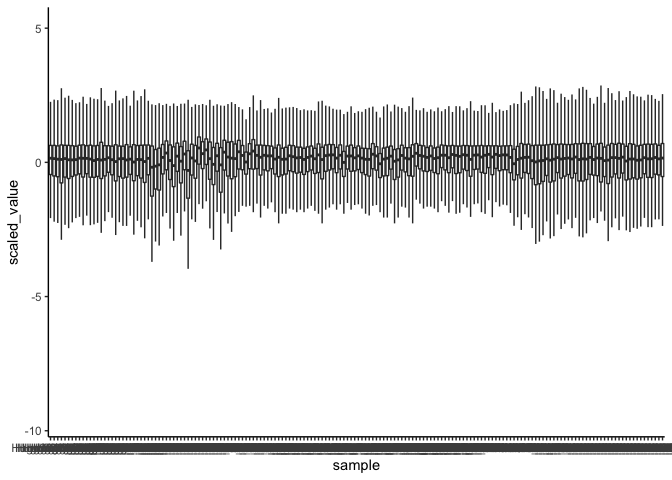
\includegraphics{explore-combined-impres-data_files/figure-latex/unnamed-chunk-3-1.pdf}

\subsection{Test gene list for differences in
response}\label{test-gene-list-for-differences-in-response}

\subsubsection{Just plot a couple of genes of interest for sitc
presentation}\label{just-plot-a-couple-of-genes-of-interest-for-sitc-presentation}

Of 8 genes of interest, 8 are represented by gene symbol in the IMPRES
set.

For each of those, compute ANOVA for linear model, with dataset and
objective\_response as effects.

P-values for the genes of interest

P-value

PDCD1

0.06440

GZMB

0.06620

LAG3

0.06985

PRF1

0.07895

CD274

0.09495

CD8A

0.09949

CTLA4

0.13931

HAVCR2

0.20372

Plots for each gene
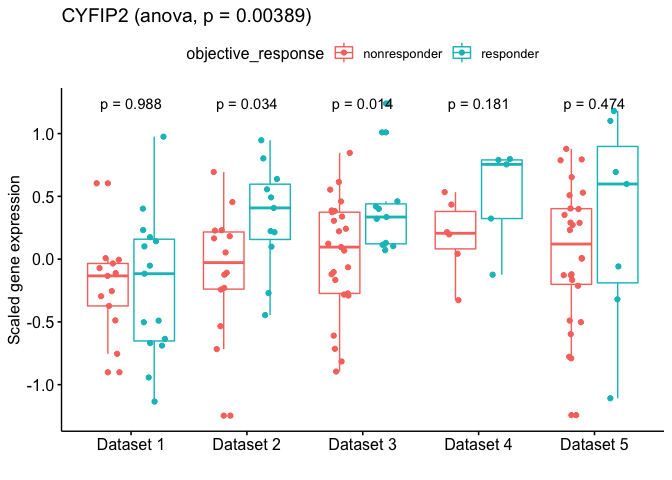
\includegraphics{explore-combined-impres-data_files/figure-latex/unnamed-chunk-9-1.pdf}
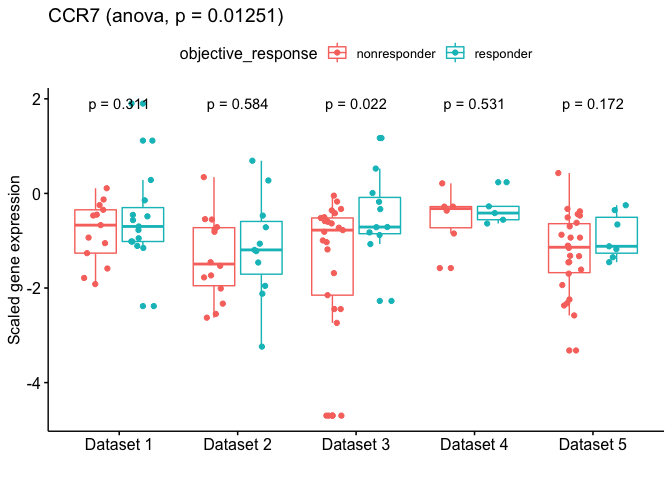
\includegraphics{explore-combined-impres-data_files/figure-latex/unnamed-chunk-9-2.pdf}
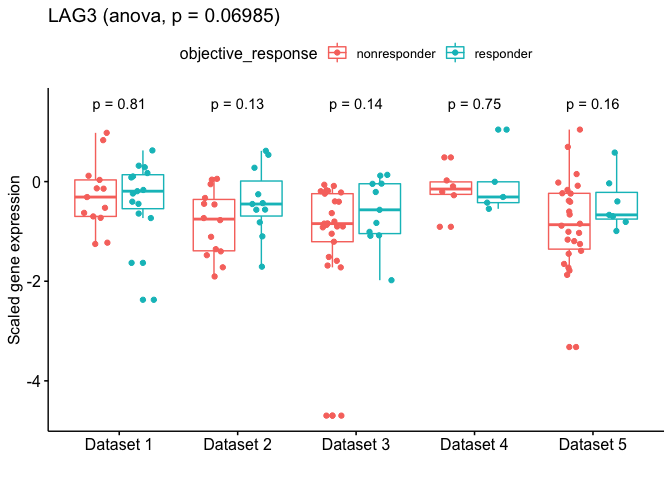
\includegraphics{explore-combined-impres-data_files/figure-latex/unnamed-chunk-9-3.pdf}
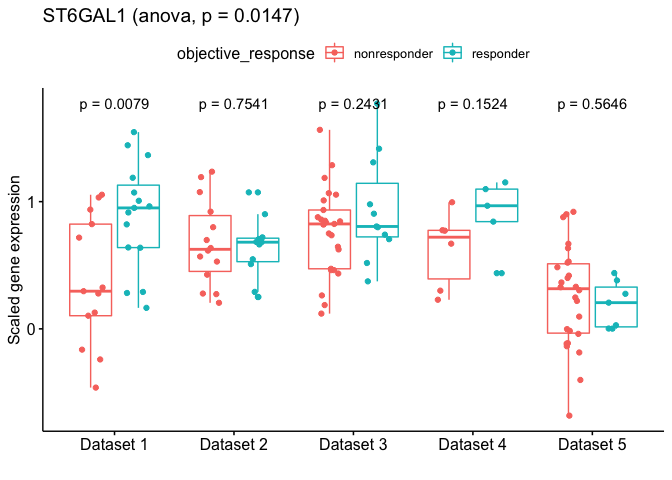
\includegraphics{explore-combined-impres-data_files/figure-latex/unnamed-chunk-9-4.pdf}
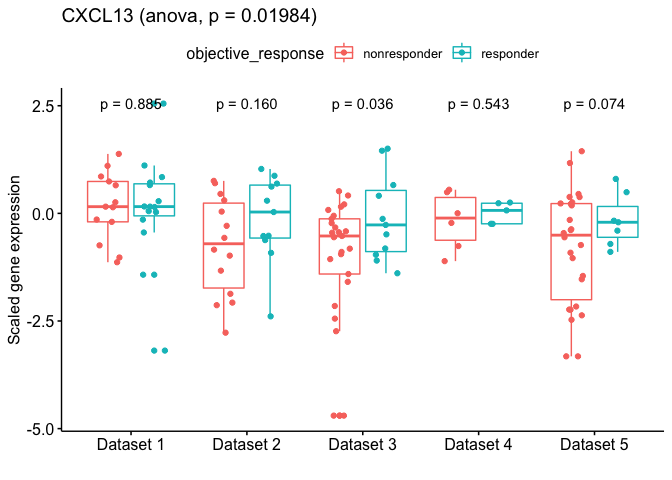
\includegraphics{explore-combined-impres-data_files/figure-latex/unnamed-chunk-9-5.pdf}
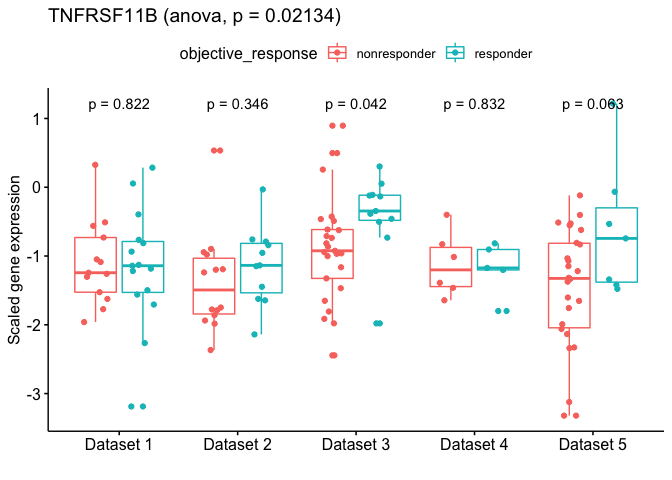
\includegraphics{explore-combined-impres-data_files/figure-latex/unnamed-chunk-9-6.pdf}
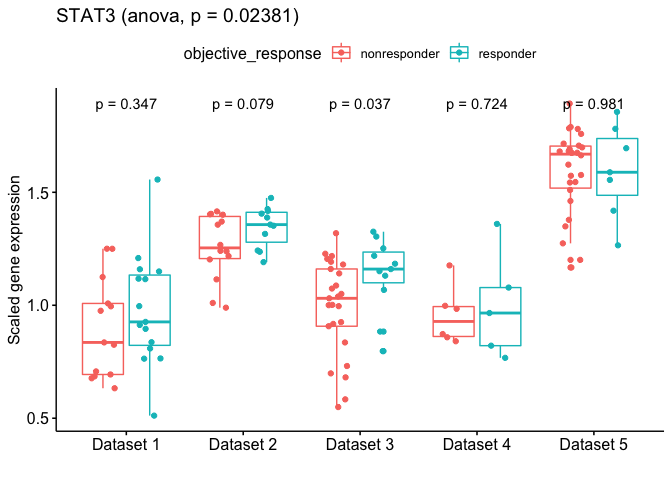
\includegraphics{explore-combined-impres-data_files/figure-latex/unnamed-chunk-9-7.pdf}
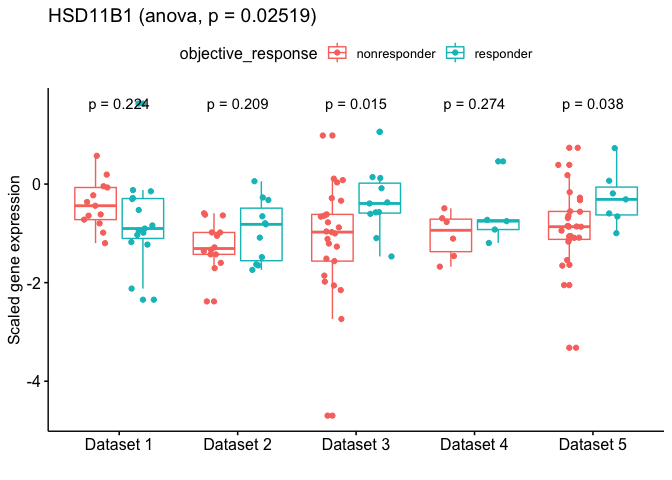
\includegraphics{explore-combined-impres-data_files/figure-latex/unnamed-chunk-9-8.pdf}

\subsubsection{Longer list}\label{longer-list}

Of 715 genes of interest, 551 are represented by gene symbol in the
IMPRES set.

For each of those, compute ANOVA for linear model, with dataset and
objective\_response as effects.

Lowest p-values

P-value

CYFIP2

0.00389

CCR7

0.01251

NFKB2

0.01308

ST6GAL1

0.01470

CXCL13

0.01984

TNFRSF11B

0.02134

STAT3

0.02381

HSD11B1

0.02519

IL21R

0.03024

IL2RA

0.03321

CD3E

0.03585

SELE

0.03623

BCL6

0.03764

CARD11

0.04001

FLT3

0.04090

IL17RA

0.04130

IRF1

0.04222

NFKB1

0.04280

TLR8

0.04307

LTB

0.04324

Plots for top genes

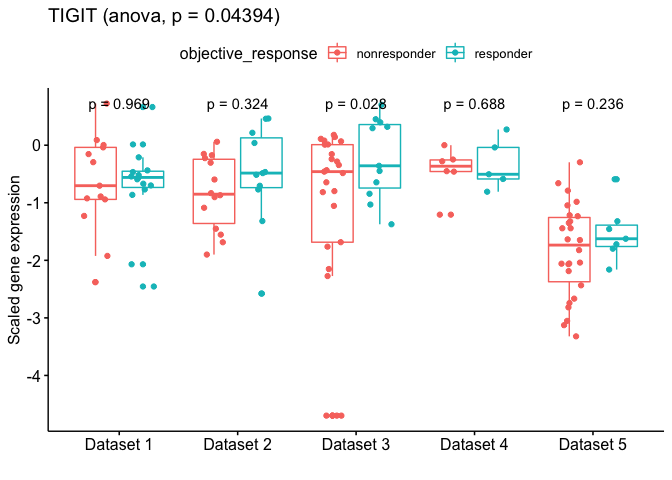
\includegraphics{explore-combined-impres-data_files/figure-latex/unnamed-chunk-13-1.pdf}
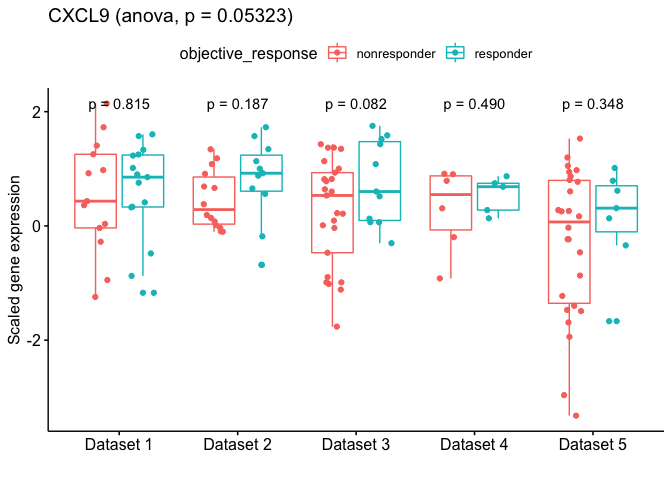
\includegraphics{explore-combined-impres-data_files/figure-latex/unnamed-chunk-13-2.pdf}
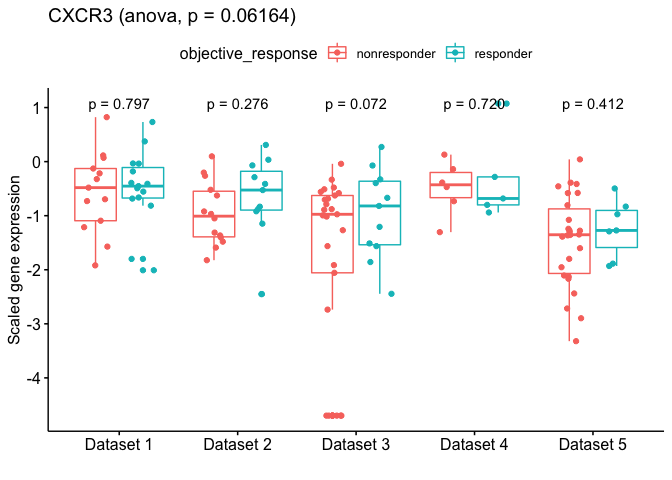
\includegraphics{explore-combined-impres-data_files/figure-latex/unnamed-chunk-13-3.pdf}
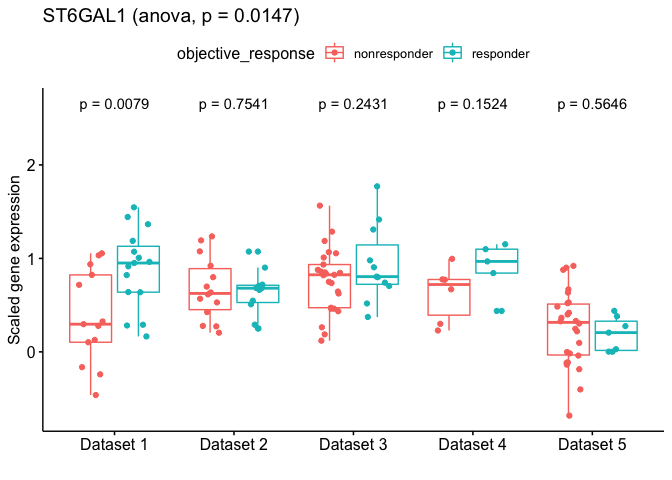
\includegraphics{explore-combined-impres-data_files/figure-latex/unnamed-chunk-13-4.pdf}
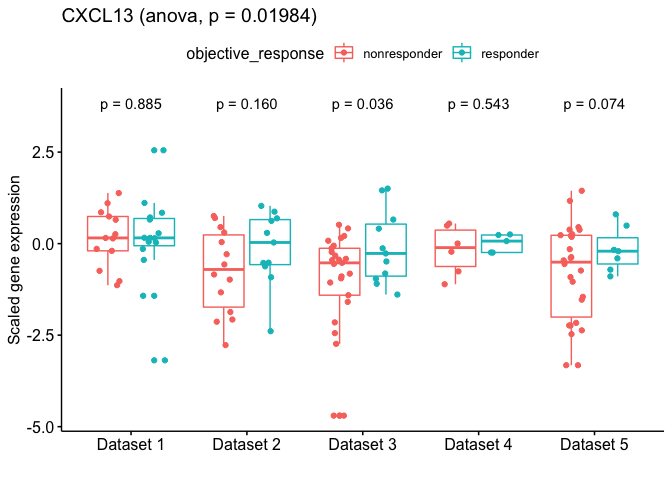
\includegraphics{explore-combined-impres-data_files/figure-latex/unnamed-chunk-13-5.pdf}
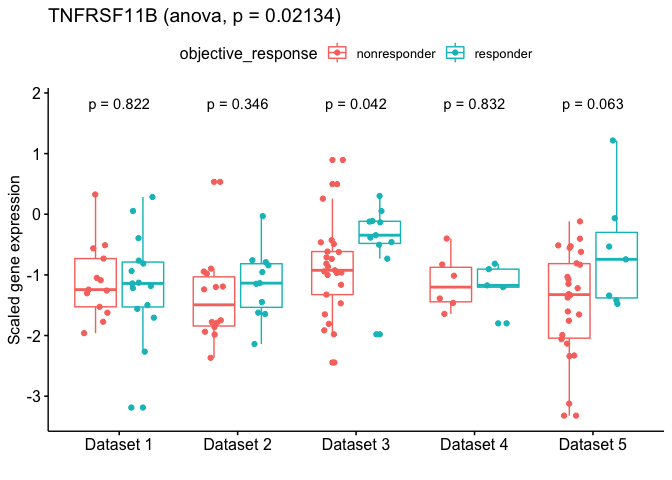
\includegraphics{explore-combined-impres-data_files/figure-latex/unnamed-chunk-13-6.pdf}
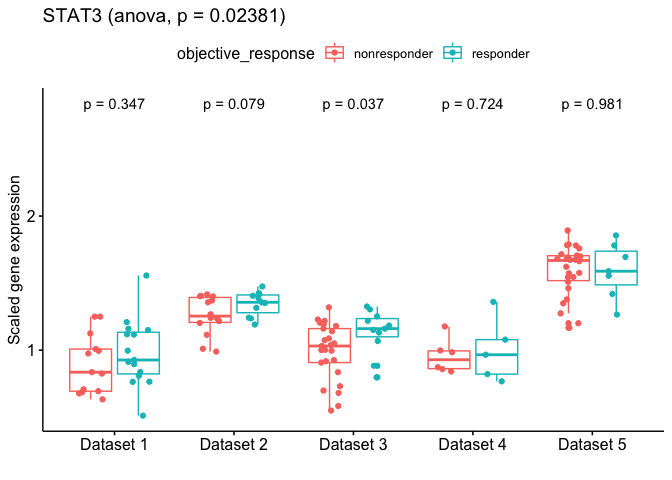
\includegraphics{explore-combined-impres-data_files/figure-latex/unnamed-chunk-13-7.pdf}
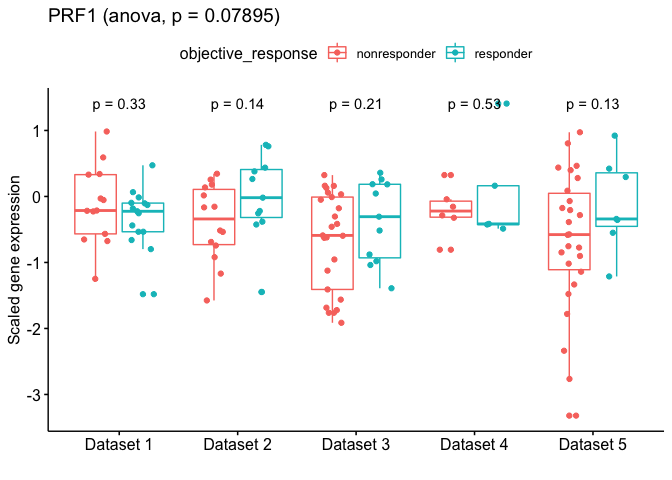
\includegraphics{explore-combined-impres-data_files/figure-latex/unnamed-chunk-13-8.pdf}
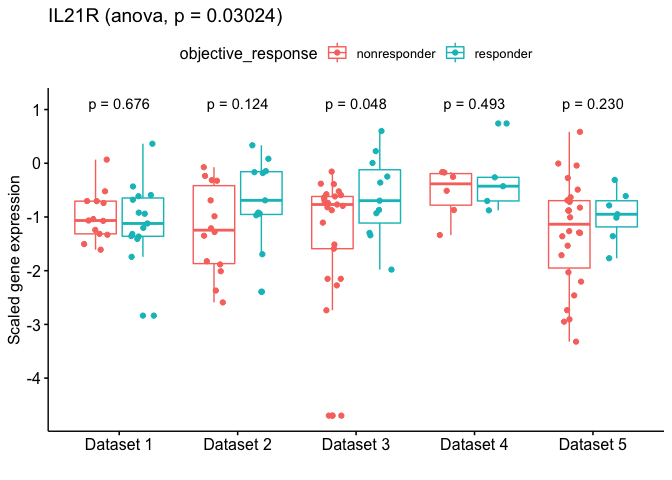
\includegraphics{explore-combined-impres-data_files/figure-latex/unnamed-chunk-13-9.pdf}
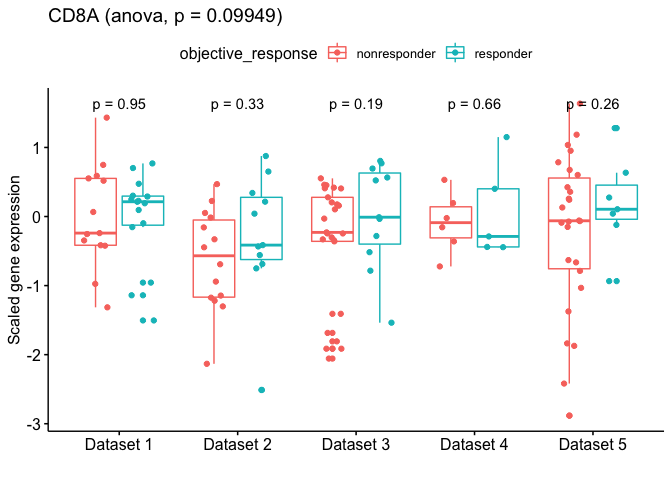
\includegraphics{explore-combined-impres-data_files/figure-latex/unnamed-chunk-13-10.pdf}
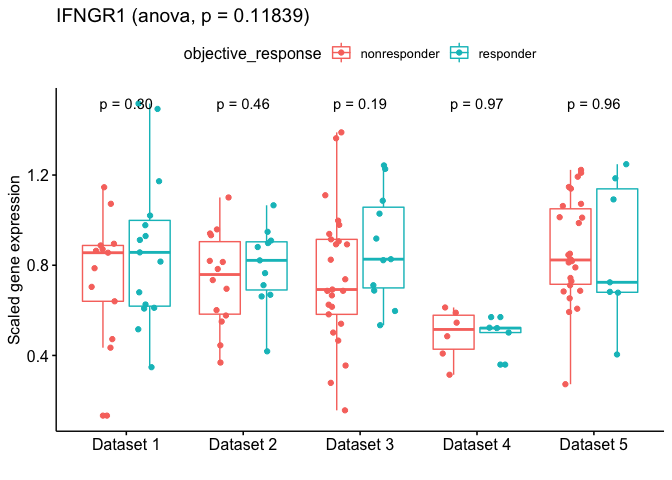
\includegraphics{explore-combined-impres-data_files/figure-latex/unnamed-chunk-13-11.pdf}
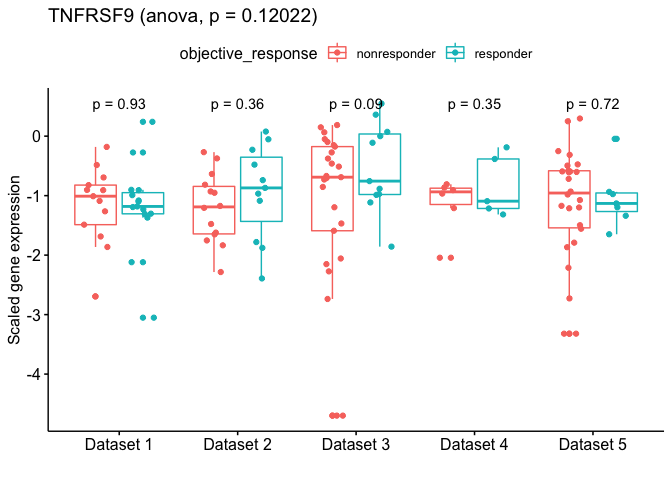
\includegraphics{explore-combined-impres-data_files/figure-latex/unnamed-chunk-13-12.pdf}
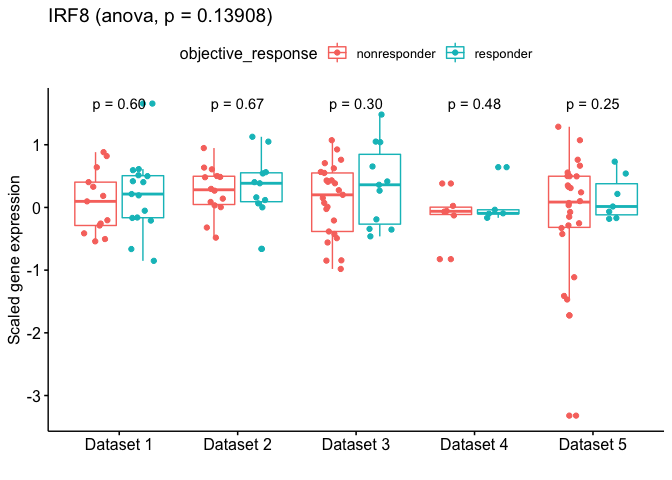
\includegraphics{explore-combined-impres-data_files/figure-latex/unnamed-chunk-13-13.pdf}
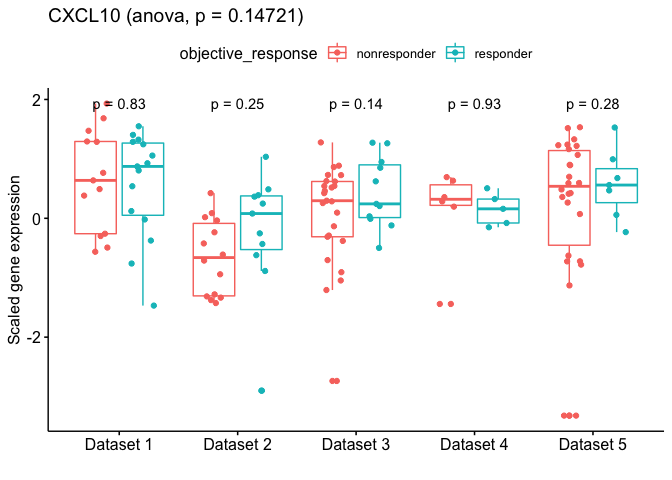
\includegraphics{explore-combined-impres-data_files/figure-latex/unnamed-chunk-13-14.pdf}
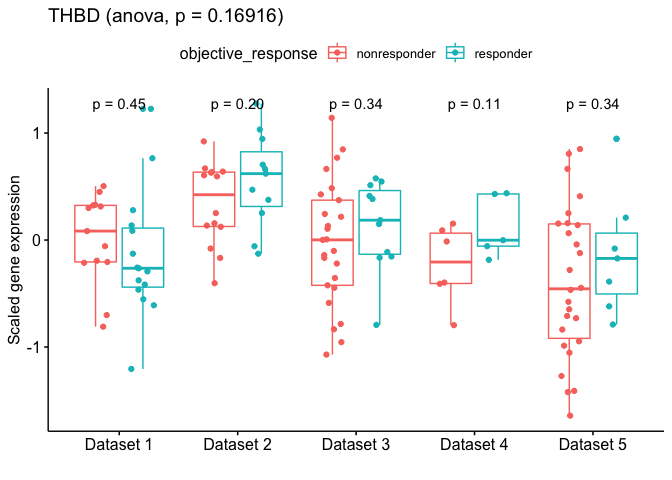
\includegraphics{explore-combined-impres-data_files/figure-latex/unnamed-chunk-13-15.pdf}
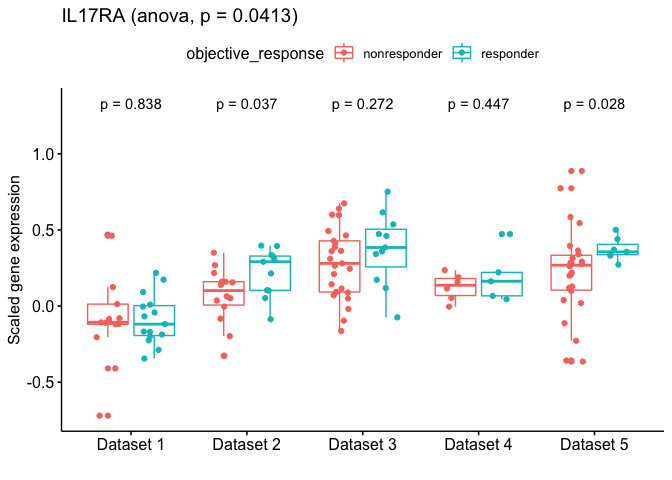
\includegraphics{explore-combined-impres-data_files/figure-latex/unnamed-chunk-13-16.pdf}
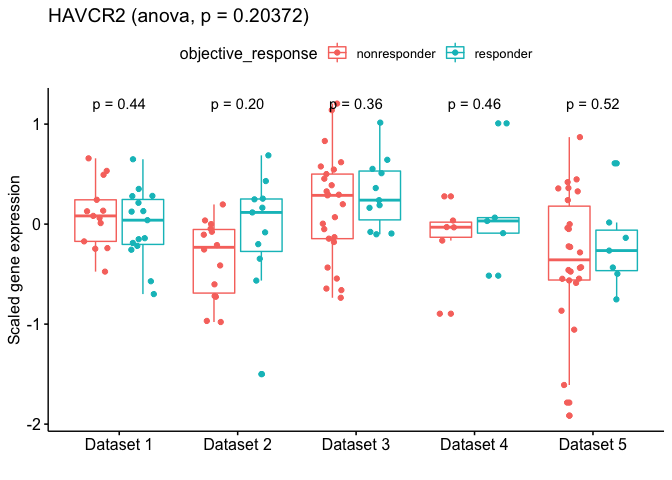
\includegraphics{explore-combined-impres-data_files/figure-latex/unnamed-chunk-13-17.pdf}
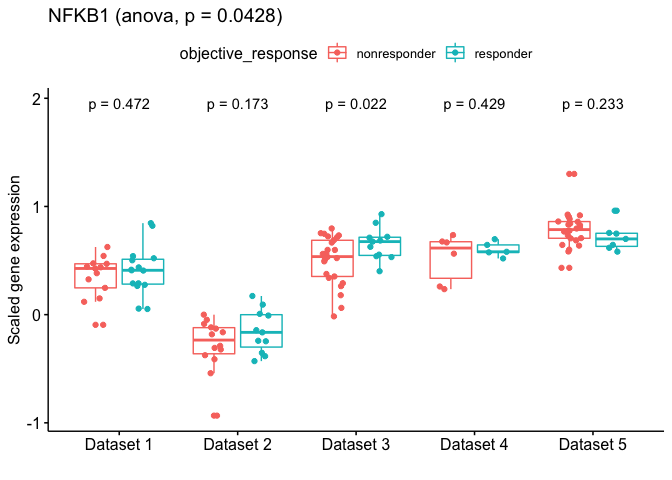
\includegraphics{explore-combined-impres-data_files/figure-latex/unnamed-chunk-13-18.pdf}
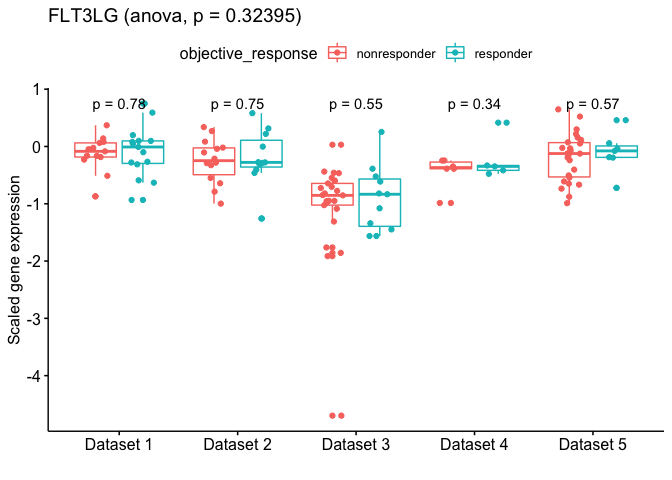
\includegraphics{explore-combined-impres-data_files/figure-latex/unnamed-chunk-13-19.pdf}
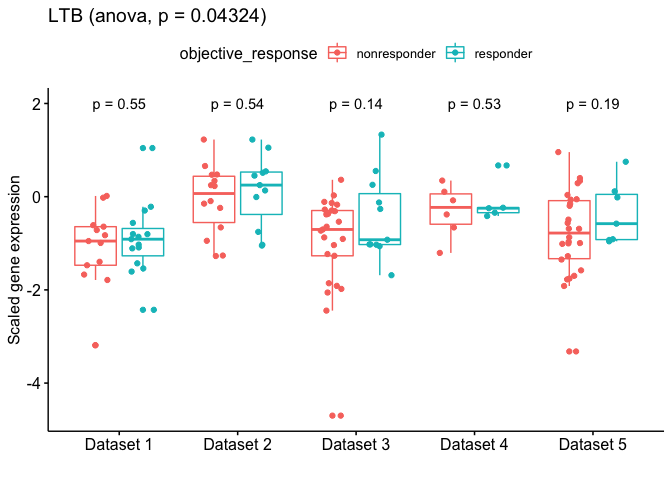
\includegraphics{explore-combined-impres-data_files/figure-latex/unnamed-chunk-13-20.pdf}

\subsubsection{More focused list}\label{more-focused-list}

Of 34 genes of interest, 27 are represented by gene symbol in the IMPRES
set.

For each of those, compute ANOVA for linear model, with dataset and
objective\_response as effects.

P-values for the genes of interest

P-value

TIGIT

0.04394

CXCL9

0.05323

CXCR3

0.06164

PDCD1

0.06440

GZMB

0.06620

LAG3

0.06985

IDO1

0.07000

PRF1

0.07895

CD274

0.09495

CD8A

0.09949

IFNGR1

0.11839

TNFRSF9

0.12022

IRF8

0.13908

CXCL10

0.14721

THBD

0.16916

GZMA

0.18311

HAVCR2

0.20372

CCL5

0.23928

FLT3LG

0.32396

IFNGR2

0.34578

ITGAM

0.50607

XCL1

0.52420

BATF3

0.55156

NT5E

0.63707

ENTPD1

0.74859

TGFB1

0.78055

ITGAE

0.82085

Plots for each gene
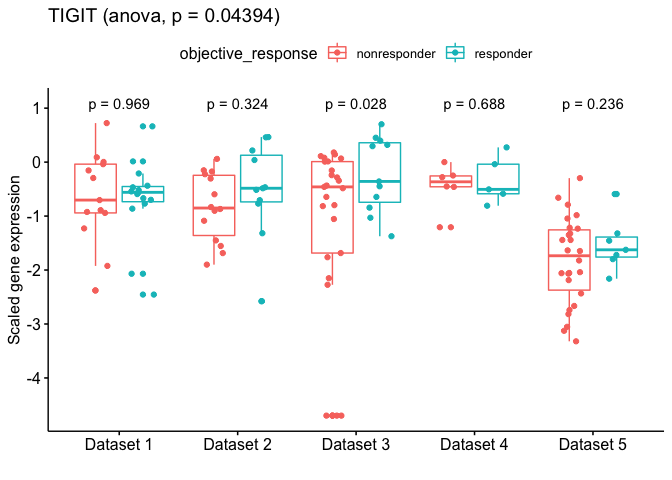
\includegraphics{explore-combined-impres-data_files/figure-latex/unnamed-chunk-17-1.pdf}
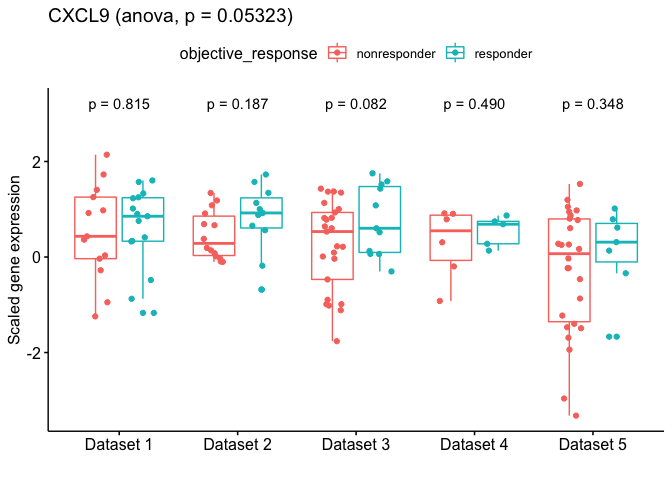
\includegraphics{explore-combined-impres-data_files/figure-latex/unnamed-chunk-17-2.pdf}
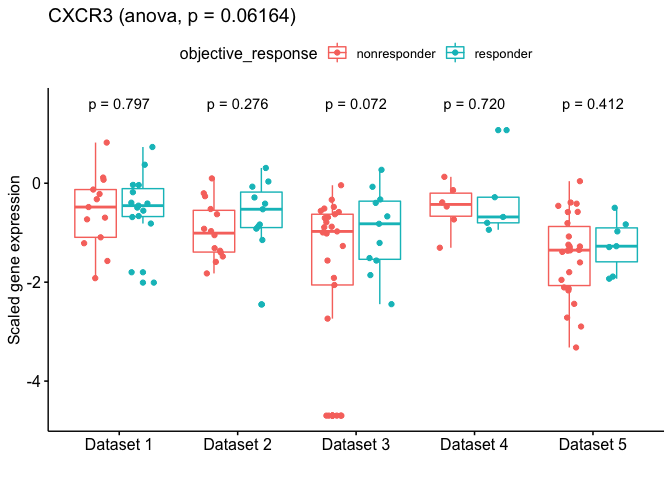
\includegraphics{explore-combined-impres-data_files/figure-latex/unnamed-chunk-17-3.pdf}
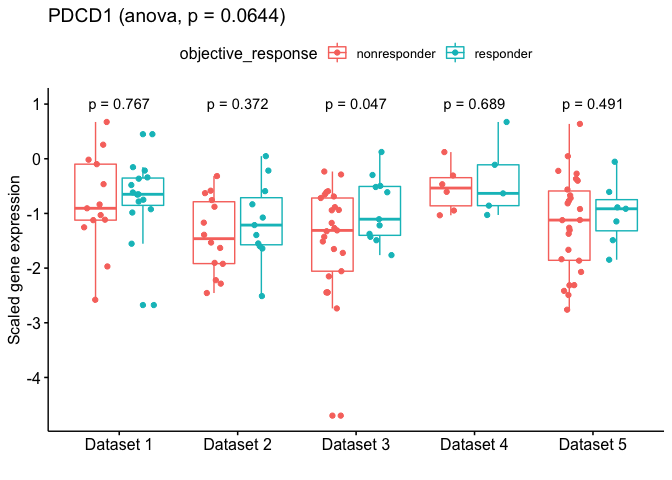
\includegraphics{explore-combined-impres-data_files/figure-latex/unnamed-chunk-17-4.pdf}
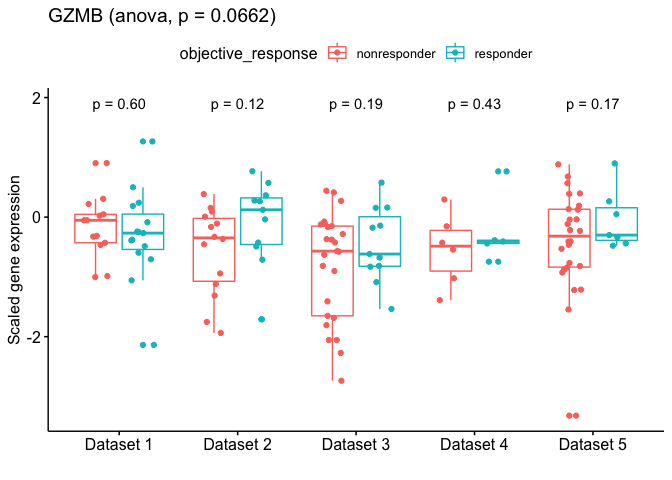
\includegraphics{explore-combined-impres-data_files/figure-latex/unnamed-chunk-17-5.pdf}
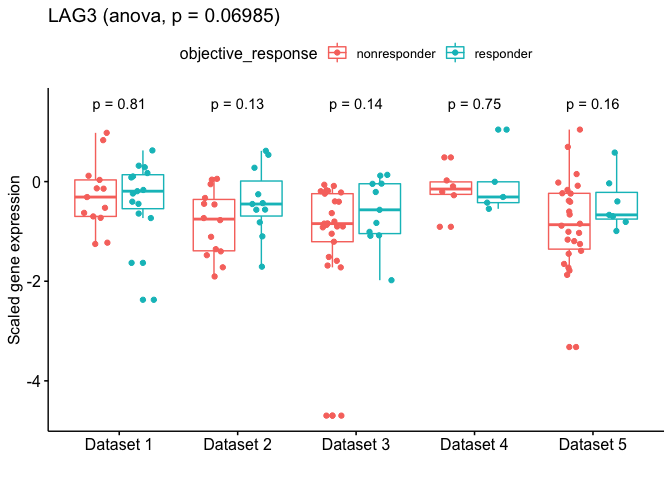
\includegraphics{explore-combined-impres-data_files/figure-latex/unnamed-chunk-17-6.pdf}
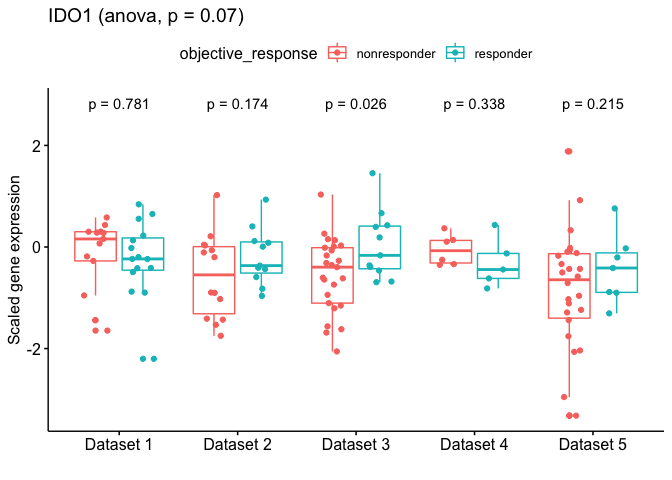
\includegraphics{explore-combined-impres-data_files/figure-latex/unnamed-chunk-17-7.pdf}
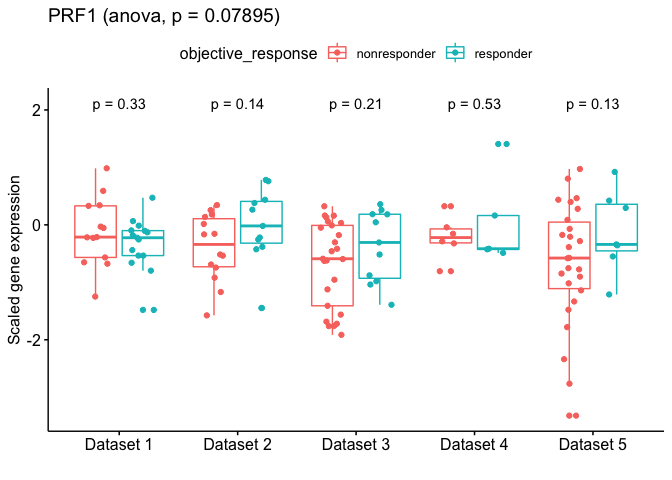
\includegraphics{explore-combined-impres-data_files/figure-latex/unnamed-chunk-17-8.pdf}
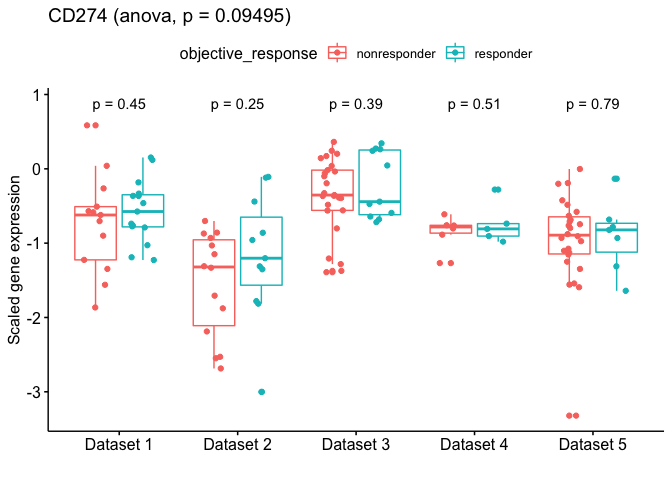
\includegraphics{explore-combined-impres-data_files/figure-latex/unnamed-chunk-17-9.pdf}
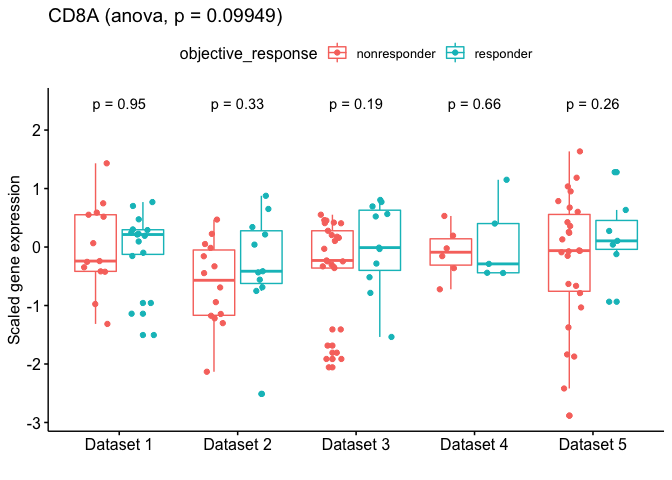
\includegraphics{explore-combined-impres-data_files/figure-latex/unnamed-chunk-17-10.pdf}
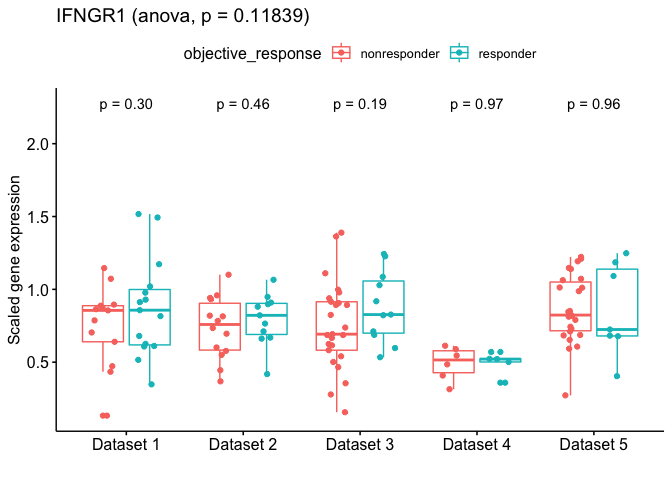
\includegraphics{explore-combined-impres-data_files/figure-latex/unnamed-chunk-17-11.pdf}
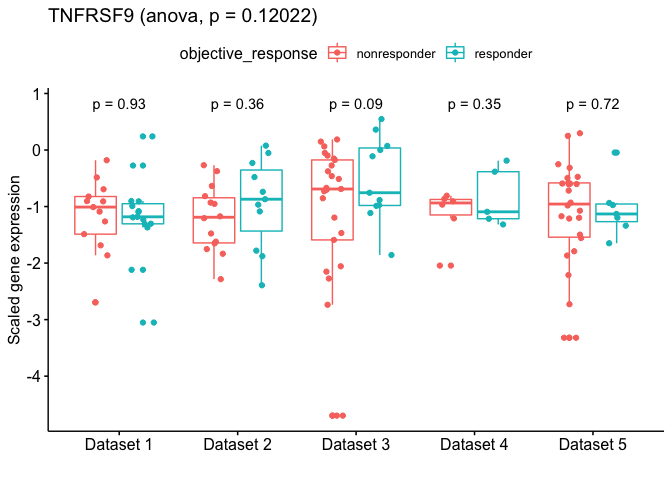
\includegraphics{explore-combined-impres-data_files/figure-latex/unnamed-chunk-17-12.pdf}
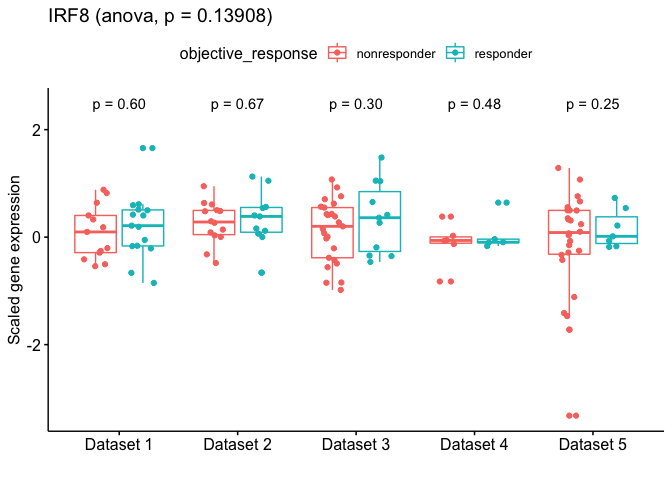
\includegraphics{explore-combined-impres-data_files/figure-latex/unnamed-chunk-17-13.pdf}
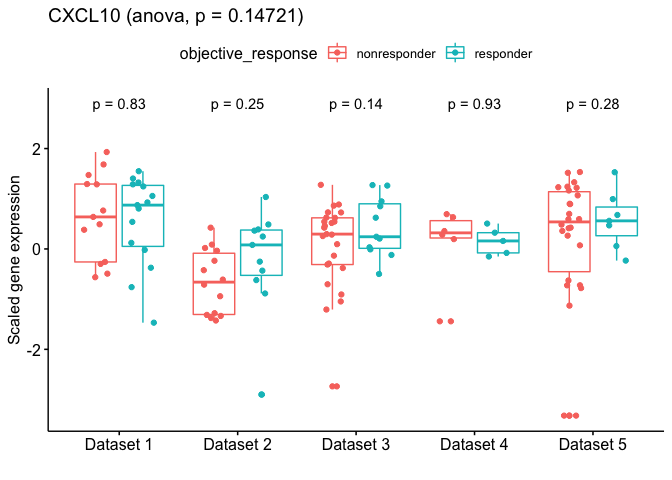
\includegraphics{explore-combined-impres-data_files/figure-latex/unnamed-chunk-17-14.pdf}
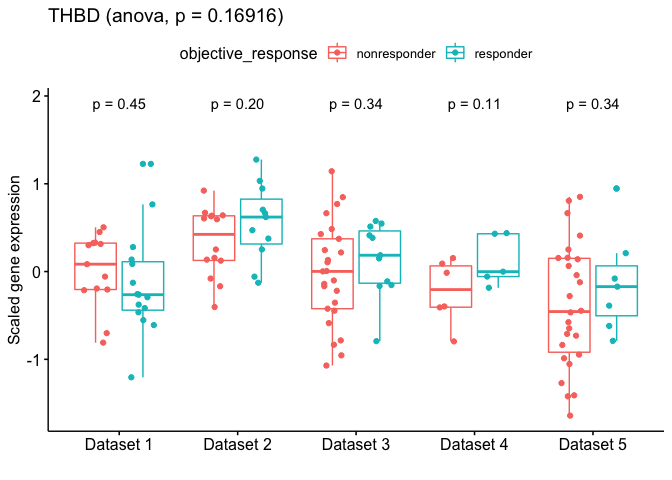
\includegraphics{explore-combined-impres-data_files/figure-latex/unnamed-chunk-17-15.pdf}
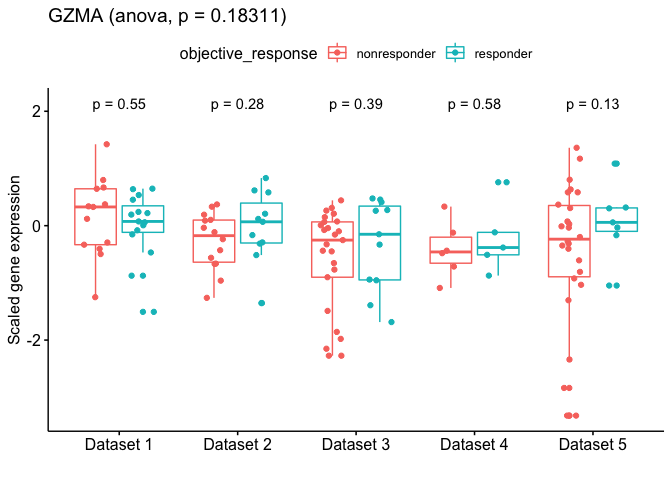
\includegraphics{explore-combined-impres-data_files/figure-latex/unnamed-chunk-17-16.pdf}
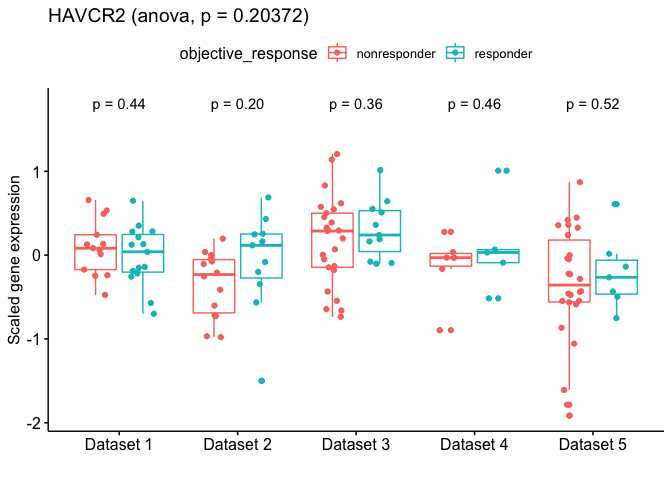
\includegraphics{explore-combined-impres-data_files/figure-latex/unnamed-chunk-17-17.pdf}
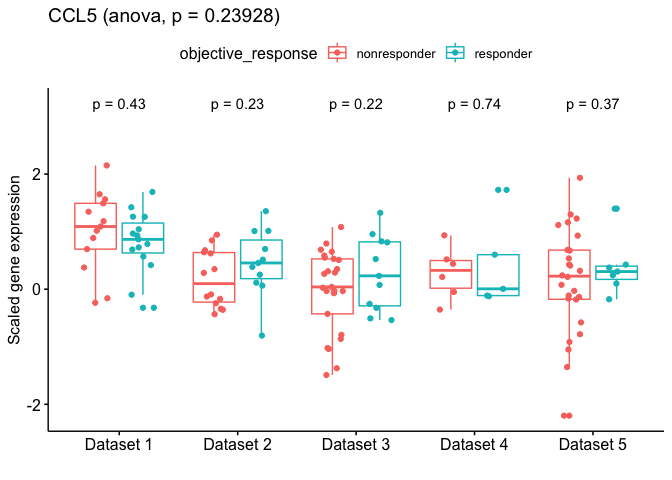
\includegraphics{explore-combined-impres-data_files/figure-latex/unnamed-chunk-17-18.pdf}
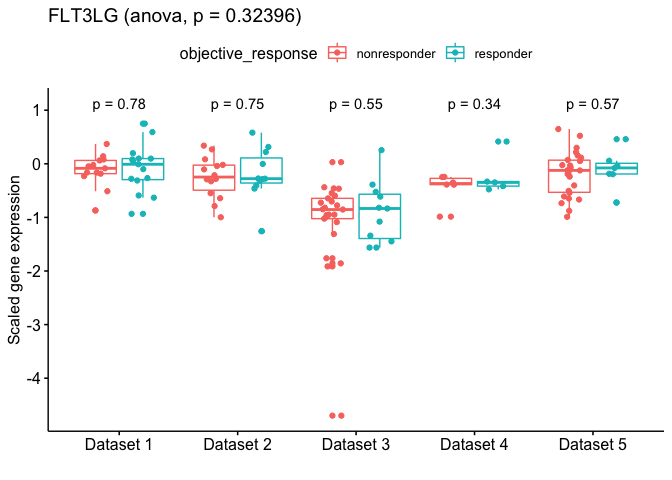
\includegraphics{explore-combined-impres-data_files/figure-latex/unnamed-chunk-17-19.pdf}
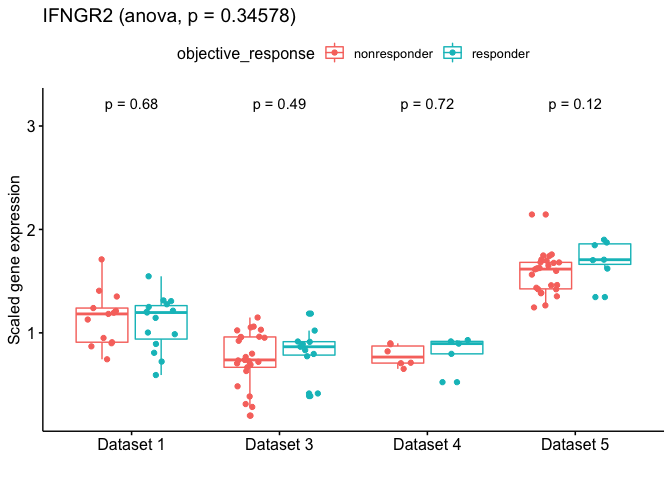
\includegraphics{explore-combined-impres-data_files/figure-latex/unnamed-chunk-17-20.pdf}
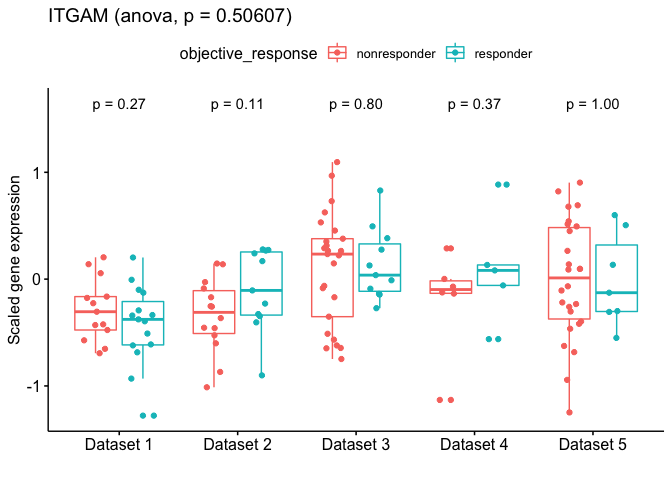
\includegraphics{explore-combined-impres-data_files/figure-latex/unnamed-chunk-17-21.pdf}
\includegraphics{explore-combined-impres-data_files/figure-latex/unnamed-chunk-17-22.pdf}
\includegraphics{explore-combined-impres-data_files/figure-latex/unnamed-chunk-17-23.pdf}
\includegraphics{explore-combined-impres-data_files/figure-latex/unnamed-chunk-17-24.pdf}
\includegraphics{explore-combined-impres-data_files/figure-latex/unnamed-chunk-17-25.pdf}
\includegraphics{explore-combined-impres-data_files/figure-latex/unnamed-chunk-17-26.pdf}
\includegraphics{explore-combined-impres-data_files/figure-latex/unnamed-chunk-17-27.pdf}


\end{document}
